\documentclass[10pt]{beamer}
\usetheme{Antibes}
\usepackage[utf8]{vietnam} 
% \usepackage[vietnam]{babel}
\usepackage{ragged2e}
% \usepackage[T1]{fontenc}

\usepackage{graphicx}


%Global Background must be put in preamble
% \usebackgroundtemplate%
% {%
%     
\includegraphics[height=\paperheight,width=\paperwidth]{backgr2.png}%
% }

%---------------end package for background image
\usepackage{graphicx}
\usepackage[dvips]{color}
% coding styles  %%%%%%%%%% font for code terminal
% \setbeamercovered{transparent}
\usepackage{listings}
\usepackage{xcolor}
 
\definecolor{codegreen}{rgb}{0,0.6,0}
\definecolor{codegray}{rgb}{0.5,0.5,0.5}
\definecolor{codepurple}{rgb}{0.58,0,0.82}
\definecolor{backcolour}{rgb}{0.95,0.95,0.92}
 
\lstdefinestyle{mystyle}{
    backgroundcolor=\color{backcolour},   
    commentstyle=\color{codegreen},
    keywordstyle=\color{magenta},
    numberstyle=\tiny\color{codegray},
    stringstyle=\color{codepurple},
    basicstyle=\ttfamily\footnotesize,
    breakatwhitespace=false,         
    breaklines=true,                 
    captionpos=b,                    
    keepspaces=true,                 
    numbers=left,                    
    numbersep=5pt,                  
    showspaces=false,                
    showstringspaces=false,
    showtabs=false,                  
    tabsize=2
}
 
\lstset{style=mystyle}
 
% end coding styles
\title{Flappy Bird}
\subtitle{AI Presentation}
\author{Team 21}
\institute{HUST}
\date{\today}
\usetheme{Boadilla}


\begin{document}
{
\usebackgroundtemplate{
\includegraphics[height=\paperheight, width=\paperwidth]{backgr2.png}}%
\begin{frame}{\textbf{AI PRESENTATION}}
    \framesubtitle{Flappy bird}
    \textbf{TEAM 21}
\begin{itemize}
\item Phí Hoàng Long      20184288
\item Vũ Tùng Lâm         20184283
\item Nguyễn Văn Lực      20176812
\end{itemize}
\vspace{4cm}
\end{frame}
}
{
\usebackgroundtemplate{
\includegraphics[height=\paperheight, width=\paperwidth]{backgr2.png}}%
\begin{frame}{\textbf{FLAPPY BIRD}}
    \framesubtitle{\textbf{Introduction}}
\begin{itemize}
\item FLAPPY BIRD is a mobile game developed by a Vietnamese video game artist and programmer 
    Dong Nguyen, under his game development company dotGears.
    \pause
\item Released in May 2013 and at the end of January 2014, the most downloaded free game in Appstore.
\pause
\item Removed from Appstore and Google Play by its creator due to what he considered to be its addictive nature and overuse.
\end{itemize}
\vspace{4cm}
\end{frame}
}
{
\usebackgroundtemplate{
\includegraphics[height=\paperheight, width=\paperwidth]{backgr2.png}}%
\begin{frame}{\textbf{FLAPPY BIRD}}
    \framesubtitle{\textbf{Introduction}}
\begin{itemize}
\item A side-scrolling mobile game featuring 2D retro style graphics.
\pause 
\item The objective is to direct a flying bird, name “Faby”.
\end{itemize}
\vspace{1cm}
\pause

\includegraphics[scale=0.35]{pipes2.png}
\end{frame}
}
{
\usebackgroundtemplate{
\includegraphics[height=\paperheight, width=\paperwidth]{backgr.png}}%
\begin{frame}[fragile]{\textbf{FLAPPY BIRD}}
    \framesubtitle{\textbf{Load images and set window}}
    \begin{minipage}{0.65\textwidth}
        \begin{itemize}
            \item  Bird's status : 
\includegraphics[scale=0.7]{bird1.png} 
\includegraphics[scale=0.7]{bird2.png} 
\includegraphics[scale=0.7]{bird3.png}
            \pause 
            \item  Install \texttt{pygame, neat-python} and remove \texttt{neat} library\\
            \texttt{pip install pygame neat-python}\\
            \texttt{pip uninstall neat}
            % \item Sample implementation : 
            \begin{lstlisting}[language=Python]
        #import libraries
    import pygame
    import neat
            \end{lstlisting}
        \end{itemize}
        \vspace{2cm}
    \end{minipage}
    \begin{minipage}{0.25\textwidth}
        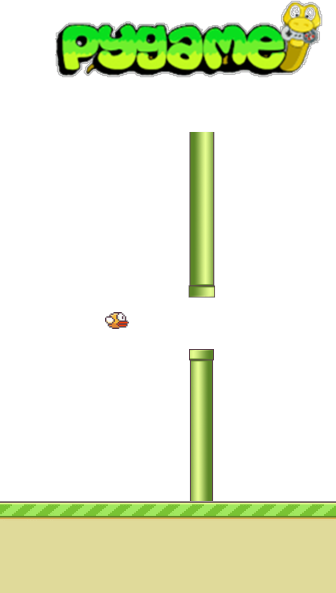
\includegraphics[scale=0.38]{pipes_ground.png}
    \end{minipage}
\end{frame}
}
{
\usebackgroundtemplate{
\includegraphics[height=\paperheight, width=\paperwidth]{backgr.png}}%
\begin{frame}[fragile]{\textbf{FLAPPY BIRD}}
    \framesubtitle{\textbf{Load images and set window}}
    \begin{itemize}
        \item Load images: \\
            \begin{lstlisting}[language=Python]
    #Load images
BIRD_IMGS = [pygame.image.load(os.path.join("img", "bird1.png")),
    pygame.image.load(os.path.join("img", "bird2.png")),
    pygame.image.load(os.path.join("img", "bird3.png"))]
PIPE_IMG = pygame.transform.scale(pygame.image.load(
    os.path.join("img", "pipe.png")), (60, 400))
BASE_IMG = pygame.transform.scale(pygame.image.load(
    os.path.join("img", "base.png")), (400, 112))
BG_IMG = pygame.transform.scale(pygame.image.load(
    os.path.join("img", "bg.png")), (400, 600))
            \end{lstlisting}
        \pause 
        \item Load windows: \\
        \begin{lstlisting}[language=Python]
    #Load window
WIN_WIDTH = 400
WIN_HEIGHT = 600
WIN = pygame.display.set_mode((WIN_WIDTH, WIN_HEIGHT))
        \end{lstlisting}
    \end{itemize}
\end{frame}
}
{
\usebackgroundtemplate{
\includegraphics[height=\paperheight, width=\paperwidth]{backgr.png}}%
\begin{frame}[fragile]{\textbf{FLAPPY BIRD}}
    \framesubtitle{\textbf{Evaluate a genome and draw window}}
    \begin{itemize}
        \item Evaluation function \\
            \begin{lstlisting}[language=Python]
    # Evaluation function
def eval_genomes(genomes, config):
    for pipe in pipes:
        for index, bird in enumerate(birds):
            if pipe.collide(bird):
                ge[index].fitness -= 1
                birds.pop(index)
                nets.pop(index)
                ge.pop(index)
            if not pipe.passed and pipe.x < bird.x:
                pipe.passed = True
                add_pipe = True
        if pipe.x + pipe.PIPE_TOP.get_width() < 0:
            rem.append(pipe)   
        pipe.move()
    if add_pipe:
        score += 1
        pipes.append(Pipe(400))
            \end{lstlisting}
    \end{itemize}
\end{frame}
}
{
\usebackgroundtemplate{
\includegraphics[height=\paperheight, width=\paperwidth]{backgr.png}}%
\begin{frame}[fragile]{\textbf{FLAPPY BIRD}}
    \framesubtitle{\textbf{Evaluate a genome and draw window}}
    \begin{itemize}
        \item Draw window \\
        \begin{lstlisting}[language=Python]
    # Draw window
def draw_window(win, birds, pipes, base, score, GEN, pipe_ind):
    if GEN == 0:
        GEN = 1
    win.blit(BG_IMG, (0,0))
    for pipe in pipes:
        pipe.draw(win)
    base.draw(win)
    for bird in birds:
        bird.draw(win)
    pygame.display.update()
        \end{lstlisting}
    \end{itemize}
\end{frame}
}
{
\usebackgroundtemplate{
\includegraphics[height=\paperheight, width=\paperwidth]{backgr.png}}%
\begin{frame}[fragile]{\textbf{FLAPPY BIRD}}
        \framesubtitle{\textbf{Genetic Algorithm}}
        \begin{definition}{Genetic algorithm}
            Genetic algorithm is a search heuristic that is inspired by Charles Darwin’s theory of natural evolution. This algorithm reflects the process of natural selection where the fittest individuals are selected for reproduction in order to produce offspring of the next generation
        \end{definition} 
        Genetic Algorithm implementation
        \begin{enumerate}
        \item Initialize the population : 
            \begin{lstlisting}[language=Python]
        p = neat.Population(config)
            \end{lstlisting}
        \pause 
        \item Create neural network for each unit : 
            \begin{lstlisting}[language=Python]
    for _,g in genomes :
        g.fitness = 0
        net = neat.nn.FeedForwardNetwork.create(g, config)
        nets.append(net)
        birds.append(Bird(150,250))
            \end{lstlisting}
        \end{enumerate}
\end{frame}
}
{
\usebackgroundtemplate{
\includegraphics[height=\paperheight, width=\paperwidth]{backgr.png}}%
\begin{frame}[fragile]{\textbf{FLAPPY BIRD}}
        \framesubtitle{\textbf{Genetic Algorithm}}
        Genetic Algorithm implementation
        \begin{enumerate}
            \setcounter{enumi}{2}
            \item Calculate the fitness-function : 
                    \begin{lstlisting}[language=Python]
        for x, bird in enumerate(birds):
            bird.move()
            ge[x].fitness += 0.1
            output = nets[x].activate((bird.y,
                abs(bird.y - pipes[pipe_ind].height),
                abs(bird.y - pipes[pipe_ind].bottom)))
            if output[0] > 0.5:
                bird.jump()
                    \end{lstlisting}
                \pause 
            \item Evaluate the current population for the next: 
                    \begin{lstlisting}[language=Python]
        # population.py
        k = 0
        while n is None or k < n:
            k += 1
            self.reporters.start_generation(self.generation)
            ... 
                    \end{lstlisting}
        \end{enumerate}
\end{frame}
}
{
\usebackgroundtemplate{
\includegraphics[height=\paperheight, width=\paperwidth]{backgr.png}}%
\begin{frame}[plain]
    \vfill
    \begin{beamercolorbox}[center]{title}
    %    example text
    
\includegraphics[scale=0.3]{tk.png}\\
    
\includegraphics[scale=1]{bird1.png}
    
\includegraphics[scale=1]{bird2.png}
    
\includegraphics[scale=1]{bird3.png}
    
    \end{beamercolorbox}
    \vfill
  \end{frame}
}

\end{document}

